\chapter{CLOUD COMPUTING}
\label{chap:cloud-computing}

\section{Cloud-Native}
\label{sec:cna}
The definition of the cloud-native term is usually related to something built on the cloud, rather than being on-premise \cite{gannon_2017}. However, this definition is incomplete, as cloud-native refers to the software method of creating, deploying, and managing modern applications in cloud computing environments \cite{aws_2025}. Therefore, it is possible to host cloud-native applications (CNAs) both in the cloud and on-premises, where both styles are sometimes used simultaneously.

The growth of microservices architecture, in conjunction with this model of hosting applications, has introduced a new level of complexity in analyzing problems within the underlying infrastructure. Where organizations once relied on centralized, monolithic systems, modern environments feature distributed frameworks characterized by containerized workloads, independently deployable microservices, and multi-cloud infrastructure arrangements \cite{bhatia_2025}.


%\lstinputlisting[language=Java, 
%caption=Texto texto texto texto
%,label=lst:exemplocodigo2]{chapters/trechos_codigo/java.m}
%\hfill
%\begin{minipage}[t]{.65\textwidth}
%\ABNTEXfontereduzida\selectfont\textbf{Fonte:}
%\end{minipage}

\section{Kubernetes}
\label{sec:k8s}

Kubernetes is a Greek word meaning ``helmsman'' or ``pilot'' \cite{luksa_2018}, or ``governor'' \cite{santos_2019}. Its conception introduced a novel approach to deploying and managing containers, especially as microservice architecture (MSA) has become more popular. The transition from monolithic applications to cloud-native microservices architectures, orchestrated by Kubernetes (K8s), has introduced significant operational complexity. Unlike traditional environments, where monitoring relied on checking the binary (up/down) states of static servers, Kubernetes manages ephemeral, dynamic containers, making failures unpredictable and challenging to diagnose with only conventional metrics \cite{usman_2022}.

In this scenario, observability transcends traditional monitoring. It is defined as the property of a system that allows its internal state to be understood from its external outputs (telemetry), enabling the correlation of signals to identify "unknown unknowns" \cite{hausenblas_2023,creane_2022}. For applications orchestrated via Kubernetes, a reference architecture should address the collection, processing, and correlation of data across multiple layers: infrastructure (nodes), orchestrator (K8s), and application (microservices).

\subsubsection{Kubernetes Architecture}

As described by \cite{brendan_tracey_2018}, although Kubernetes' conception makes it easier to deploy and manage distributed systems, Kubernetes itself is a distributed system that needs to be managed. Its architecture/cluster can be divided into two layers: the control plane and the worker plane, as seen in figure \ref{fig:k8s-arch}. Kubernetes \citeonline{kubernetes_components_2019} call these components as key to make up a K8S cluster. Given the importance of these architectural elements, it is necessary to delve into the details regarding these two components. 

\begin{figure}[ht]
    \centering
    \caption{Kubernetes Architecture}
    \label{fig:k8s-arch}
    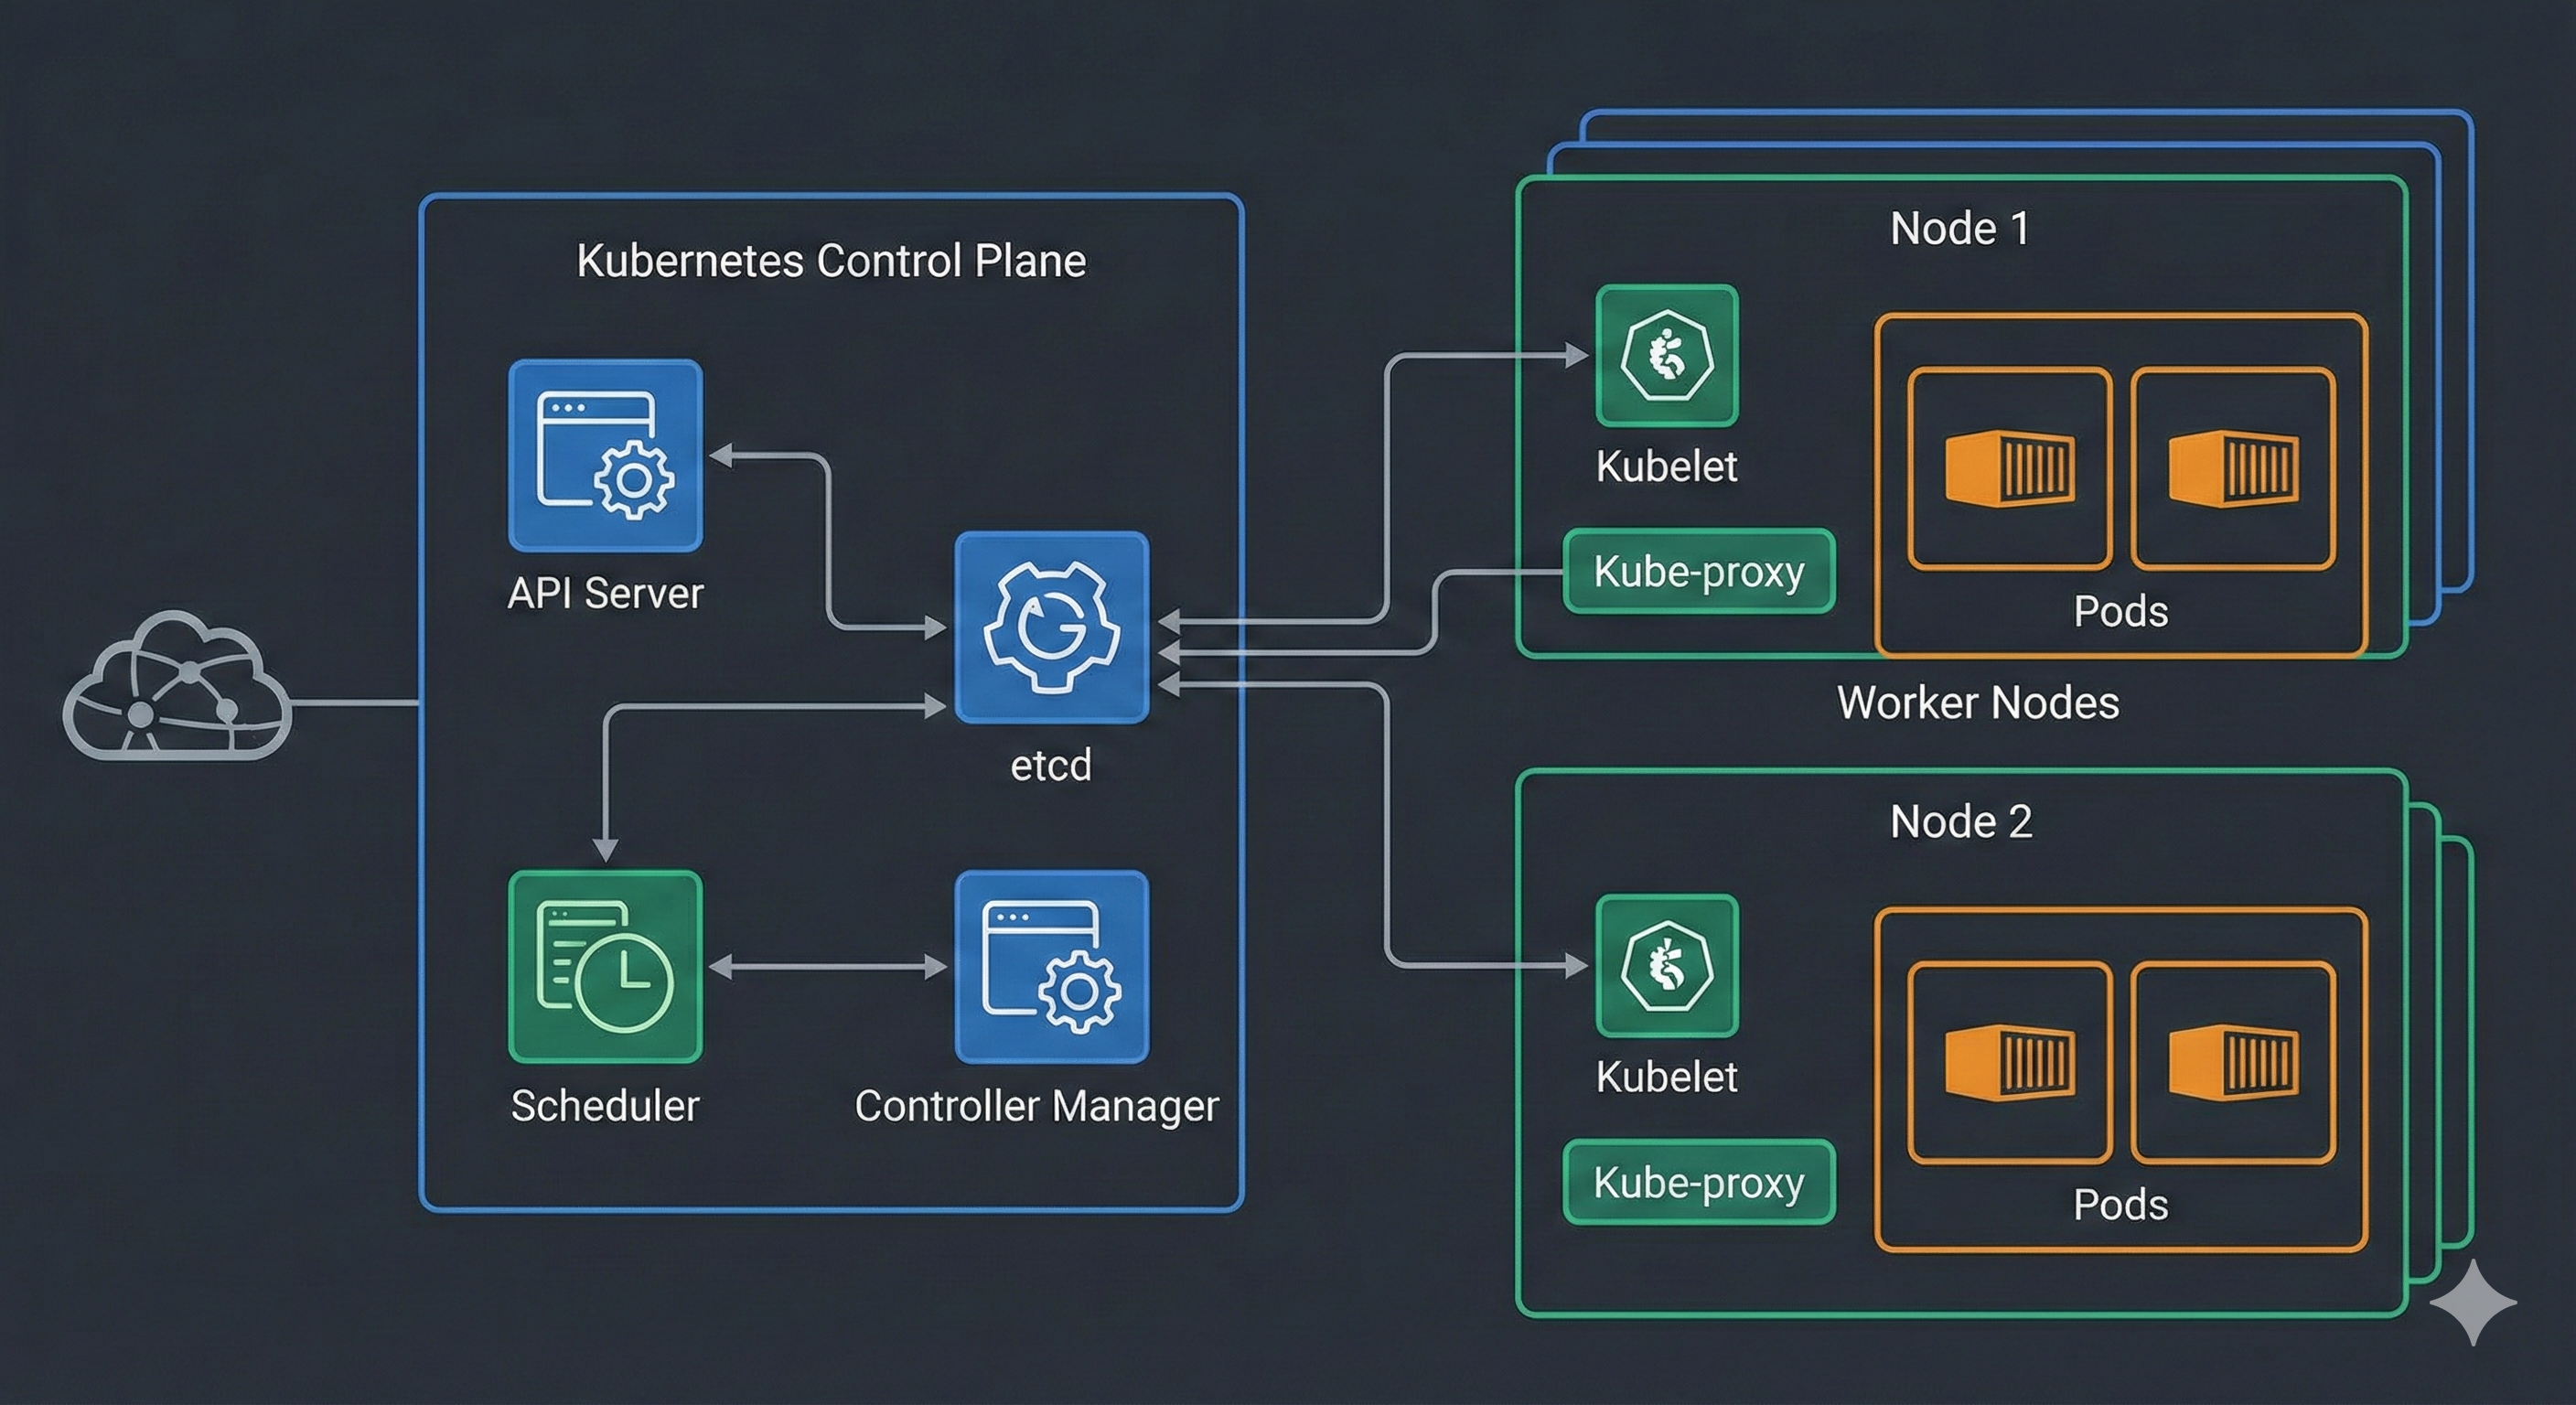
\includegraphics[width=1.0\linewidth]{images/cloud-computing/k8s-architecture.png}
    \par\medskip\ABNTEXfontereduzida\selectfont\textbf{Source:} \cite{kubernetes_2019} \par\medskip
\end{figure}

\textbf{The Control Plane}

The Control Plane is what controls the cluster and makes it function \cite{luksa_2018}. It is known as the ``brain'' of the cluster \cite{brendan_tracey_2018}. It is responsible for making global decisions (such as scheduling), detecting and responding to events (such as starting a new Pod when a replica fails), and maintaining the desired state of the system. In standard architecture diagrams (figure \ref{fig:control-plane}), it is often represented as a block containing four essential components and one optional:

\begin{figure}[ht]
    \centering
    \caption{Control Plane}
    \label{fig:control-plane}
    \includegraphics[width=1.0\linewidth]{images/cloud-computing/control-plane.png}
    \par\medskip\ABNTEXfontereduzida\selectfont\textbf{Source:} \cite{kubernetes_2019} \par\medskip
\end{figure}

\begin{itemize}
    \item API Server: The central component and the only communication interface for the Control Plane. All other components (whether the Scheduler, the Controller Manager, or the Kubelet on the nodes) communicate solely with the API Server, never directly with each other or with the database. It validates and configures data objects (Pods, Services, etc.).
    \item etcd: This is the consistent, high-availability key-value store used as the "source of truth" (backing store) for all cluster data. Kubernetes does not store state in the processing components; everything is persisted in etcd. Only the API Server has permission to read from and write to it.
    \item Scheduler: The component is responsible for resource allocation. It watches for newly created Pods that do not yet have a Node assigned and selects the best Node for them to run on, based on resource constraints (CPU/Memory), affinity policies, taints, and tolerations.
    \item Controller Manager: This component executes the control loops. It monitors the cluster's current state via the API Server and compares it with the desired state. If there is a divergence (e.g., a Pod died and the desired state specifies 3 replicas), it takes steps to correct it (e.g., creating a new Pod). It includes controllers such as the Node Controller and the Replication Controller.
    \item Cloud Control Manager: The component is responsible for integrating with cloud providers such as GCP \cite{kubernetes_components_2019}.
\end{itemize}

\textbf{Worker Nodes}

The Worker Nodes (represented as Node 1 and Node 2 in typical diagrams) are the "muscles" of the cluster. These are the machines (physical or virtual) where the workloads (applications) actually run. Each node has components to manage containers and communicate with the Control Plane:

\begin{itemize}
    \item Kubelet: The primary agent running on each node. It registers the node with the API Server and watches for Pod specifications (`PodSpecs`) assigned to that node. The Kubelet ensures that the containers described in those Pods are running and healthy, reporting their status back to the Control Plane. It also interacts with native monitoring tools, such as cAdvisor, to collect usage metrics.
    \item Kube-proxy: A network proxy running on each node. It maintains network rules (using `iptables' or `ipvs' on Linux) to allow network communication to Pods from within or outside the cluster. It enables the concept of a "Service" in Kubernetes by performing basic load balancing.
    \item Pods: Often represented as blocks containing containers, Pods are the smallest deployable unit in Kubernetes. A Pod encapsulates one or more containers (usually Docker/containerd), shared storage, and a unique IP within the cluster network.
\end{itemize}

\textbf{The Master-Worker Relationship}

The relationship between the Control Plane (historically called the Master) and the Worker Nodes is one of Command and Execution:

Unlike imperative orchestration models that rely on direct, synchronous execution of commands, the interaction between the Kubernetes Control Plane and Worker Nodes is fundamentally declarative and asynchronous \cite{burns_2016}. In this paradigm, the Control Plane does not micromanage individual node operations; instead, it persists the \textit{desired state} of the system into etcd, which serves as the single source of truth \cite{luksa_2018}.

The orchestration process follows a rigorous reconciliation loop:

\begin{enumerate}
    \item Scheduling: The \textit{kube-scheduler} evaluates resource constraints and affinity policies to assign (bind) a pending Pod to a specific Node, updating the API Server record \cite{hausenblas_2023}.
    \item Actuation: The \textit{Kubelet} daemon does not passively wait for commands. Instead, it utilizes a Watch API mechanism to continuously monitor the API Server for new specifications assigned to its node. Upon detecting a state divergence (e.g., a new Pod assignment), the Kubelet instructs the local container runtime (CRI) to align the actual state with the desired specification \cite{sayfan_2017}.
    \item Self-Healing: System resilience is maintained through continuous monitoring. If a node fails to renew its lease (heartbeat), the \textit{kube-controller-manager} detects the deviation from the desired state and automatically reschedules affected workloads to healthy nodes, ensuring state convergence without human intervention \cite{beyer_2016}.
\end{enumerate}

This separation ensures that the orchestration intelligence (Control Plane) is decoupled from the actual workload (Worker Nodes), allowing the system to be highly scalable and resilient.

\subsection{Layers of the Observability Architecture}

The proposed architecture is based on a telemetry data pipeline composed of four fundamental stages: Generation (Instrumentation), Collection, Processing/Storage, and Analysis \cite{kosinska_2023,young_2024}. These stages allow practitioners to explore and unveil errors and anomalies in applications.

However, at the instrumentation layer, there are several options for generating data. Each one of them represents a different level of analysis. Consistent with the taxonomy presented by \citeonline{he_2021}, log data in Kubernetes environments is generated across three distinct layers: Infrastructure (Node), Platform (Cluster), and Application (Workload). While structurally similar—composed of a constant template and variable parameters \cite{he_2017}—semantics vary significantly. Anomalies in this context are often characterized not just by explicit keywords such as 'fatal' or 'crash', but also by contextual tokens indicating resource exhaustion or connectivity timeouts (e.g., 'backoff', 'unreachable'), which are commonly found in distributed system datasets like HDFS and BGL \cite{du_2017}.

\subsubsection{Instrumentation and Signal Generation Layer}
The basis of observability lies in proper instrumentation. In the context of Kubernetes, it is possible to extract data from three primary sources:

\textbf{Infrastructure and Nodes (Node-level):} This involves capturing CPU, memory, disk, and network metrics from the underlying operating system. The Kubelet, the agent that runs on each node, natively includes \textit{cAdvisor}, which collects resource usage metrics from containers and exposes them for consumption \cite{burns_2019,hausenblas_2023}.

\textbf{Kubernetes Control Plane:} Components such as the API Server, Controller Manager, and Scheduler expose vital metrics and audit logs that record the sequence of activities and decisions made by the cluster, essential for security and troubleshooting \cite{creane_2022,muschko_2020}.

\textbf{Application (Microservices):} Business metrics, structured logs, and distributed traces are considered golden signals \cite{turnbull_2018}; therefore, applications should be instrumented to emit these signals. OpenTelemetry (OTel) has become the industry standard for this instrumentation, unifying signal generation without vendor dependency (vendor-agnostic) \cite{young_2024,flanders_2024}.

\subsubsection{Collection Patterns in Kubernetes}

Data collection in a Kubernetes cluster can be implemented through different architectural patterns, each with specific advantages:

\textbf{DaemonSet (Agent per Node):} This is the most efficient pattern for collecting infrastructure logs and metrics. An agent (such as Fluentd or OpenTelemetry Collector) is deployed on each node of the cluster. It reads logs directly from the `/var/log/containers` directory (or `stdout`/`stderr` streams from Docker/containerd) and collects host metrics, enriching the data with Kubernetes metadata (such as namespace, pod name, labels) \cite{wilkins_2019, creane_2022, dubey_2021}.

\textbf{Sidecar:} A sidecar container is deployed in the same Pod as the application. Although it consumes more resources, it helps convert logs from legacy applications or service mesh proxies that collect detailed network metrics \cite{burns_2019,ibryam_2019}.

\textbf{Operators (Kubernetes Operators):} The Operator pattern is widely used to manage the observability lifecycle. For example, the Prometheus Operator \cite{operator_hub_2026} or the OpenTelemetry Operator \cite{otel_operator_2026} automates configuration injection, agent management, and service discovery for metric scraping \cite{dobies_2020,flanders_2024}.

\subsubsection{Processing and Storage Layer}
Once telemetry data is collected, it must be processed and persisted effectively. In a default Kubernetes installation, data is ephemeral: metrics in the Metrics Server are in-memory \cite{muschko_2020}, and node logs are rotated. To achieve the "Storage" stage of the pipeline, the architecture must utilize Kubernetes persistence primitives.

In the processing layer, before storage, raw data often requires processing. The OpenTelemetry Collector, previously mentioned as an agent, also acts as a processor in this stage, performing batching, retry mechanisms, encryption, and data enrichment (adding cluster metadata like \textit{Pod ID} or \textit{Service Name}) to ensure context is maintained \cite{flanders_2024}.

In the storage layer, for long-term retention, observability backends (such as Prometheus for metrics or Elasticsearch/Loki for logs) are deployed as \textit{StatefulSets}. Unlike stateless applications, these components require stable network identities and persistent storage. They utilize \textbf{Persistent Volume Claims (PVCs)} mapped to a \textbf{StorageClass} to request physical storage from the underlying infrastructure (IaaS), ensuring that telemetry data survives Pod restarts or node failures \cite{luksa_2018, hausenblas_2023}.

\subsection{The Pillars of Observability in Kubernetes}

Previously, it was noted that metrics, traces, and logs are pillars of observability. In K8s, these constructs are inconsistently defined and scattered throughout its architecture for other purposes, such as the Metrics Server, which is designed to enable autoscaling. However, before elaborating on finer details of K8s, it is necessary to know its current state.

\subsubsection{Metrics and the Prometheus Ecosystem} 
For numerical time-series data, Prometheus is the \textit{de facto} standard in the Cloud Native Computing Foundation (CNCF) ecosystem \cite{yeruva_2021}. The reference architecture uses the pull model, where the Prometheus server performs the scraping of metrics exposed by the `/metrics` endpoints of the services and Kubernetes itself (via kube-state-metrics) \cite{dubey_2021}.

For horizontal pod scalability (HPA - Horizontal Pod Autoscaler), the Metrics Server is an essential component that aggregates resource usage metrics and makes them available via the Kubernetes metrics API \cite{muschko_2020}.

\subsubsection{Logs and Centralized Aggregation}
In distributed environments, logs cannot be accessed in isolation via `kubectl logs' in production. The architecture requires a log forwarder (such as Fluentd or Fluent Bit) to centralize output streams. These logs must be processed to extract structured fields correlated with Kubernetes metadata before being sent to a storage backend (such as Elasticsearch, Loki, or OpenSearch) \cite{wilkins_2019,ibryam_2019}.

\subsubsection{Distributed Tracing}
To understand latency and request flow between microservices, distributed tracing is mandatory. Tools like Jaeger or Tempo receive spans generated by applications instrumented via OpenTelemetry. The OpenTelemetry Collector component plays a crucial role here, receiving traces via protocols such as OTLP, processing them (e.g., sampling and filtering sensitive data), and exporting them to the visualization backend \cite{hausenblas_2023,young_2024}.

\subsubsection{The Role of OpenTelemetry (OTel) in the Architecture}
OpenTelemetry (OTel) acts as the unifying layer in the reference architecture. It solves the problem of tool fragmentation by providing a single standard for APIs, SDKs, and protocols (OTLP) \cite{flanders_2024}.

A central component is the OpenTelemetry Collector, which can be deployed in two main modes in Kubernetes: Agent Mode (DaemonSet) or Gateway Mode (Deployment). In the first case, it runs on each node to collect logs and metrics from the host, minimizing network latency. In the second one, it is a centralized cluster of collectors that receives data from the agents, performs heavy processing (such as tail-based sampling and aggregation), and exports to the back.

OpenTelemetry has become so relevant that cloud vendors like Google have adopted the OTLP protocol to create their own telemetry API \cite{google_cloud_observability_2024}.
\section{INFRASTRUCTURE AS CODE}
\label{sec:iac}

As cloud computing introduced the capability to provision resources via APIs (Application Programming Interfaces), the traditional manual approach to system administration became a bottleneck. Infrastructure as Code (IaC) emerged as the solution to this scalability challenge. Defined by \citeonline{morris_2016}, IaC is the practice of managing and provisioning computing infrastructure through machine-readable definition files, rather than through physical hardware configuration or interactive configuration tools.

Fundamentally, IaC applies software engineering principles—such as version control, testing, and Continuous Integration (CI)—to infrastructure operations. This paradigm shift ensures that the environment is idempotent, meaning that applying the same configuration multiple times will always result in the same system state, eliminating the "configuration drift" common in manually managed servers.

\subsection{Historical Evolution: From Snowflakes to Cattle}

The evolution of IaC is often described through the metaphor of "Pets vs. Cattle," popularized in the context of cloud architecture by \cite{bias_2016}. In the traditional model (pre-cloud), servers were treated as "Pets": they were given unique names, manually nursed to health when sick, and were difficult to replace. This led to what \citeonline{fowler_2013} describes as "Snowflake Servers"—unique, fragile systems whose configuration cannot be reproduced automatically.

With the advent of virtualization and IaaS, the paradigm shifted to "Cattle": servers are given automated identifiers, are built from a standard image, and if one fails, it is replaced rather than repaired. This evolution occurred in three phases:

\begin{enumerate}
    \item \textbf{Scripting Era:} System administrators used imperative shell scripts (Bash, Perl) to automate tasks. While better than manual input, these scripts were often brittle and hard to maintain.
    \item \textbf{Configuration Management:} Tools like Puppet, Chef, and Ansible introduced declarative languages to manage the state of operating systems, ensuring consistency across fleets of servers \cite{spinellis_2012}.
    \item \textbf{Immutable Infrastructure:} With containers and Kubernetes, the focus shifted from updating servers to replacing them entirely. Tools like Terraform and Helm allow the definition of the entire datacenter and application stack as code.
\end{enumerate}

\subsection{IaC in the Context of this Research}

In the context of this thesis, IaC is not merely an operational convenience but a methodological requirement for scientific validity. To answer the research questions regarding the effectiveness of the proposed observability architecture (PANOPTES), the experimental environment must be strictly reproducible.

We utilize IaC in two distinct layers:
\begin{itemize}
    \item \textbf{Infrastructure Layer (Ansible):} To provision the baseline environment (IaaS simulation) using Vagrant, ensuring that the underlying virtual machines have identical kernel configurations and resource limits for both the control and experimental groups.
    \item \textbf{Application Layer (Helm):} To define the reference architecture itself. The PANOPTES architecture is packaged as Helm Charts, allowing the complex orchestration of Prometheus, Jaeger, and OpenTelemetry components to be instantiated deterministically. 
\end{itemize}

This ensures that the reference architecture is an artifact that can be audited, versioned, and shared with the community, preventing the ``t works on my machine'' bias.